\week{January 24, 1993}


Well, this week I have had guests and have not been keeping up with the literature. So ``this week's finds'' are mostly papers that have been sitting around in my office and that I am now filing away.

\find{\paper{Link invariants for intersecting loops, by Daniel Armand Ugon, Rodolfo Gambini, and Pablo Mora, \href{http://cds.cern.ch/record/566149/files/9212137.pdf}{October 1992 preprint}, available from Gambini, Instituto de F\'isica, Facultad de Ciencias, Trist\'an Narvaja 1674, Montevideo, Uruguay.}}

The authors generalize the standard trick for getting link invariants from solutions of the Yang--Baxter equations, and show how to get link invariants applicable to generalized links with 4-valent or 6-valent vertices, that is, transverse double points, like
\begin{center}
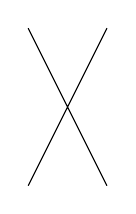
\begin{tikzpicture}
% These nodes will be reused in the next three tikzpicture environments.
\node[coordinate] (topleft) at (0,2) {};
\node[coordinate] (topright) at (1,2) {};
\node[coordinate] (botleft) at (0,0) {};
\node[coordinate] (botright) at (1,0) {};
\node (middle) at (0.5,1) {};

\draw (topleft) -- (botright)  (botleft) -- (topright);
\end{tikzpicture},
\end{center}
and transverse triple points. This involves working with a generalization of the braid group that includes generators for these vertices as well as the usual generators for crossings. In this case of 4-valent vertices, rigorously working out the generators and relations was done by Joan Birman in the paper below, but various people had used the answer already. The case of triple points is very important in physics due to the connection with the loop representation of quantum gravity (which is what Gambini is working on these days). In this representation, states are invariants of (possibly generalized) links, and only by considering links with triple points can one define operators such as the ``total volume of the universe''.

It is thus quite interesting that the authors make progress on determining the ``right'' extension of the HOMFLY polynomial invariant of links to links with transverse triple points -- that is, the extension that one gets by doing calculations in SU(n) Chern--Simons theory. In a special case, namely when the HOMFLY polynomial reduces to the Kauffman bracket (which corresponds to the Lie group SU(2)), one gets a state of quantum gravity that has been under extensive investigation these days. The authors compute the Kaufmann bracket of links with triple points using first order perturbation theory in Chern--Simons theory. A nonperturbative calculation would be very good to have!

\find{\paper{New points of view in knot theory, by Joan Birman, \href{https://arxiv.org/abs/math/9304209}{preprint}, to appear in the Bulletin of the AMS.}}

This is a nice review of the recent work on Vassiliev invariants of links. Given an invariant of oriented links, one can extend it to links with arbitrarily many double points by setting the value of the invariant on a link with a double point
\begin{center}
\begin{tikzpicture}
\draw (topleft) -- (botright)  (botleft) -- (topright);
\end{tikzpicture}
\end{center}
to be the invariant of the link with the double point changed to
\begin{center}
\begin{tikzpicture}
\draw (topleft) -- (middle) -- (botright)  (botleft) -- (topright);
\end{tikzpicture}
\end{center}
minus the invariant of the link with the double point changed to
\begin{center}
\begin{tikzpicture}
\draw (topleft) -- (botright)  (botleft) -- (middle) -- (topright);
\end{tikzpicture}.
\end{center}
Note that the link has to be oriented for this rule to make sense, and the strands shown in the pictures above should be pointing downwards. Now, having made this extension, we say a link invariant is a Vassiliev invariant of degree n if it vanishes on all links with n+1 or more double points.

It is interesting that this rule for extending link invariants to links with double points, when applied to the Kauffman bracket, does not give the extension computed by Gambini et al.\ in the paper above. (This is not surprising, actually, but it shows that some interesting things are going on in the subject of invariants for links with self-intersections and Chern--Simons theory.)

\find{\paper{Link polynomials and a graphical calculus, by Louis Kauffman and P. Vogel, \href{https://www.worldscientific.com/doi/abs/10.1142/S021821651240007X}{Jour. of Knot Theory and its Ramifications, 1 (1992), 59--104}.}}

This is another nice treatment of link invariants for generalized links with self-intersections. It concentrates on the famous link invariants coming from Chern--Simons theory -- the HOMFLY polynomial (from SU(n)) and the Kauffman polynomial (from SO(n)). Lots of good pictures.

And, switching back to the category theory, 2-categories, and the like, let me list these before filing them away:

\find{\paper{Categorical physics, by Louis Crane, preprint available as \href{https://arxiv.org/abs/hep-th/9301061}{arXiv:hep-th/9301061} in amstex.}
\paper{A Categorical construction of 4d topological quantum field theories, by Louis Crane and David Yetter, preprint available as \href{https://arxiv.org/abs/hep-th/9301062}{arXiv:hep-th/9301062} in latex.}
\paper{Hopf Categories and their representations, Louis Crane and Igor Frenkel, draft version.}
\paper{Categorification and the construction of topological quantum field theory, Louis Crane and Igor Frenkel, draft version.}}

These outline Louis Crane's vision of an approach to generally covariant 4-dimensional quantum field theories (e.g. quantum gravity or a ``theory of everything'') based on 2-categories. ``Categorical physics'' sketches the big picture, while the paper with Yetter provides a juicy mathematical spinoff -- the first known four-dimensional TQFT, based on the representations of quantum SU(2) and very similar in spirit to the Turaev--Viro construction of a 3d TQFT from quantum SU(2). The papers with Frenkel (apparently still not in their final form) describe the game plan and hint at marvelous things still to come. The conjecture is stated: ``a 4d TQFT can be reconstructed from a tensor 2-category''. This follows up on Crane's earlier work on getting 3d TQFTs from modular tensor categories (big example: the categories of representations of quantum groups at roots of unity). And the authors define the notion of a Hopf category, show how the category of module categories of a Hopf category is a tensor 2-category, and use ``categorification'' to turn the universal enveloping algebra of a quantum group into a Hopf category. Sound abstract? Indeed it is. But the aim is clear: to cook up 4d TQFTs from quantum groups. Such quantum field theories might be physically important; indeed, the one associated to SU(2) is likely to have a lot to do with quantum gravity.

I am currently perusing Kapranov and Voevodsky's massive paper on 2-categories, which seems to be the starting point for Crane's above papers and also those of Carter/Saito that I mentioned last week. Next week I should post an outline of what this paper does.

\find{\paper{The origin of time asymmetry, by S W Hawking, R Laflamme and G W Lyons, preprint available as \href{https://arxiv.org/abs/gr-qc/9301017}{arXiv:gr-qc/9301017}, in tex.}}

I haven't had a chance to read this one yet but it looks very ambitious and is likely to be interesting. Let me just quote from the introduction to get across the goal:

\begin{quote}
The laws of physics do not distinguish the future from the past direction of time. More precisely, the famous CPT theorem says that the laws are invariant under the combination of charge conjugation, space inversion and time reversal. In fact effects that are not invariant under the combination CP are very weak, so to a good approximation, the laws are invariant under the time reversal operation T alone. Despite this, there is a very obvious difference between the future and past directions of time in the universe we live in. One only has to see a film run backward to be aware of this.

There are are several expressions of this difference. One is the so-called psychological arrow, our subjective sense of time, the fact that we remember events in one direction of time but not the other. Another is the electromagnetic arrow, the fact that the universe is described by retarded solutions of Maxwell's equations and not advanced ones. Both of these arrows can be shown to be consequences of the thermodynamic arrow, which says that entropy is increasing in one direction of time. It is a non trivial feature of our universe that it should have a well defined thermodynamic arrow which seems to point in the same direction everywhere we can observe. Whether the direction of the thermodynamic arrow is also constant in time is something we shall discuss shortly.

There have been a number of attempts to explain why the universe should have a thermodynamic arrow of time at all. Why shouldn't the universe be in a state of maximum entropy at all times? And why should the direction of the thermodynamic arrow agree with that of the cosmological arrow, the direction in which the universe is expanding? Would the thermodynamic arrow reverse, if the universe reached a maximum radius and began to contract?

Some authors have tried to account for the arrow of time on the basis of dynamic laws. The discovery that CP invariance is violated in the decay of the K meson, inspired a number of such attempts but it is now generally recognized that CP violation can explain why the universe contains baryons rather than anti baryons, but it can not explain the arrow of time. Other authors have questioned whether quantum gravity might not violate CPT, but no mechanism has been suggested. One would not be satisfied with an ad hoc CPT violation that was put in by hand.

The lack of a dynamical explanation for the arrow of time suggests that it arises from boundary conditions. The view has been expressed that the boundary conditions for the universe are not a question for Science, but for Metaphysics or Religion. However that objection does not apply if there is a sense in which the universe has no boundary. We shall therefore investigate the origin of the arrow of time in the context of the no boundary proposal of Hartle \& Hawking. This was formulated in terms of Einsteinian gravity which may be only a low energy effective theory arising from some more fundamental theory such as superstrings. Presumably it should be possible to express a no boundary condition in purely string theory terms but we do not yet know how to do this. However the recent COBE observations indicate that the perturbations that lead to the arrow of time arise at a time during inflation when the energy density is about $10^{-12}$ of the Planck density. In this regime, Einstein gravity should be a good approximation.
\end{quote}

[I'll skip some more technical stuff on the validity of perturbative calculations in quantum gravity...]

\begin{quote}
One can estimate the wave functions for the perturbation modes by considering complex metrics and scalar fields that are solutions of the Einstein equations whose only boundary is the surface $S$. When $S$ is a small three sphere, the complex metric can be close to that of part of a Euclidean four sphere. In this case the wave functions for the tensor and scalar modes correspond to them being in their ground state. As the three sphere $S$ becomes larger, these complex metrics change continuously to become almost Lorentzian. They represent universes with an initial period of inflation driven by the potential energy of the scalar field. During the inflationary phase the perturbation modes remain in their ground states until their wave lengths become longer than the horizon size. The wave function of the perturbations then remains frozen until the horizon size increases to be more than the wave length again during the matter dominated era of expansion that follows the inflation. After the wave lengths of the perturbations come back within the horizon, they can be treated classically.

This behaviour of the perturbations can explain the existence and direction of the thermodynamic arrow of time. The density perturbations when they come within the horizon are not in a general state but in a very special state with a small amplitude that is determined by the parameters of the inflationary model, in this case, the mass of the scalar field. The recent observations by COBE indicate this amplitude is about $10^{-5}$. After the density perturbations come within the horizon, they will grow until they cause some regions to collapse as proto-galaxies and clusters. The dynamics will become highly non linear and chaotic and the coarse grained entropy will increase. There will be a well defined thermodynamic arrow of time that points in the same direction everywhere in the universe and agrees with the direction of time in which the universe is expanding, at least during this phase.

The question then arises: If and when the universe reaches and maximum size, will the thermodynamic arrow reverse? Will entropy decrease and the universe become smoother and more homogeneous during the contracting phase?
\end{quote}

[I'll skip some stuff on why Hawking originally thought entropy had to decrease during the Big Crunch if the no-boundary proposal were correct... and why he no longer thinks so.]

\begin{quote}
The thermodynamic arrow will agree with the cosmological arrow for half the history of the universe, but not for the other half. So why is it that we observe them to agree? Why is it that entropy increases in the direction that the universe is expanding? This is really a situation in which one can legitimately invoke the weak anthropic principle because it is a question of where in the history of the universe conditions are suitable for intelligent life. The inflation in the early universe implies that the universe will expand for a very long time before it contracts again. In fact, it is so long that the stars will have all burnt out and the baryons will have all decayed. All that will be left in the contracting phase will be a mixture of electrons, positrons, neutrinos and gravitons. This is not a suitable basis for intelligent life.
The conclusion of this paper is that the no boundary proposal can explain the existence of a well defined thermodynamic arrow of time. This arrow always points in the same direction. The reason we observe it to point in the same direction as the cosmological arrow is that conditions are suitable for intelligent life only at the low entropy end of the universe's history.
\end{quote}
